\documentclass[12pt,twoside]{article}
\usepackage[dvipsnames]{xcolor}
\usepackage{tikz,graphicx,amsmath,amsfonts,amscd,amssymb,mathrsfs, bm,cite,epsfig,epsf,url}
\usepackage[hang,flushmargin]{footmisc}
\usepackage[colorlinks=true,urlcolor=blue,citecolor=blue]{hyperref}
\usepackage{amsthm,multirow,wasysym,appendix}
\usepackage{array,subcaption} 
% \usepackage[small,bf]{caption}
\usepackage{bbm}
\usepackage{pgfplots}
\usetikzlibrary{spy}
\usepgfplotslibrary{external}
\usepgfplotslibrary{fillbetween}
\usetikzlibrary{arrows,automata}
\usepackage{thmtools}
\usepackage{blkarray} 
\usepackage{textcomp}
\usepackage{float}
\usepackage[left=0.8in,right=1.0in,top=1.0in,bottom=1.0in]{geometry}


\usepackage{times}
\usepackage{amsfonts}
\usepackage{amsmath}
\usepackage{latexsym}
\usepackage{color}
\usepackage{graphics}
\usepackage{enumerate}
\usepackage{amstext}
\usepackage{blkarray}
\usepackage{url}
\usepackage{epsfig}
\usepackage{bm}
\usepackage{hyperref}
\hypersetup{
    colorlinks=true,
    linkcolor=blue,
    filecolor=magenta,      
    urlcolor=blue,
}
\usepackage{textcomp}
\usepackage[left=0.8in,right=1.0in,top=1.0in,bottom=1.0in]{geometry}
\usepackage{mathtools}
%\usepackage{minted}
\usepackage{gensymb}


%% Probability operators and functions
%
% \def \P{\mathrm{P}}
\def \P{\mathrm{P}}
\def \E{\mathrm{E}}
\def \Var{\mathrm{Var}}
\let\var\Var
\def \Cov {\mathrm{Cov}} \let\cov\Cov
\def \MSE {\mathrm{MSE}} \let\mse\MSE
\def \sgn {\mathrm{sgn}}
\def \R {\mathbb{R}}
\def \C {\mathbb{C}}
\def \N {\mathbb{N}}
\def \Z {\mathbb{Z}}
\def \cV {\mathcal{V}}
\def \cS {\mathcal{S}}

\newcommand{\RR}{\ensuremath{\mathbb{R}}}

\DeclareMathOperator*{\argmin}{arg\,min}
\DeclareMathOperator*{\argmax}{arg\,max}
\newcommand{\red}[1]{\textcolor{red}{#1}}
\newcommand{\blue}[1]{\textcolor{blue}{#1}}
\newcommand{\green}[1]{\textcolor{ForestGreen}{ #1}}
\newcommand{\fuchsia}[1]{\textcolor{RoyalPurple}{ #1}}



%
%% Probability distributions
%
%\def \Bern    {\mathrm{Bern}}
%\def \Binom   {\mathrm{Binom}}
%\def \Exp     {\mathrm{Exp}}
%\def \Geom    {\mathrm{Geom}}
% \def \Norm    {\mathcal{N}}
%\def \Poisson {\mathrm{Poisson}}
%\def \Unif    {\mathrm {U}}
%
\DeclareMathOperator{\Norm}{\mathcal{N}}

\newcommand{\bdb}[1]{\textcolor{red}{#1}}

\newcommand{\ml}[1]{\mathcal{ #1 } }
\newcommand{\wh}[1]{\widehat{ #1 } }
\newcommand{\wt}[1]{\widetilde{ #1 } }
\newcommand{\conj}[1]{\overline{ #1 } }
\newcommand{\rnd}[1]{\tilde{ #1 } }
\newcommand{\rv}[1]{ \rnd{ #1}  }
\newcommand{\rx}{\rnd{ x}  }
\newcommand{\ry}{\rnd{ y}  }
\newcommand{\rz}{\rnd{ z}  }
\newcommand{\ra}{\rnd{ a}  }
\newcommand{\rb}{\rnd{ b}  }
\newcommand{\rpc}{\widetilde{ pc}  }
\newcommand{\rndvec}[1]{\vec{\rnd{#1}}}

\def \cnd {\, | \,}
\def \Id { I }
\def \J {\mathbf{1}\mathbf{1}^T}

\newcommand{\op}[1]{\operatorname{#1}}
\newcommand{\setdef}[2]{ := \keys{ #1 \; | \; #2 } }
%\newcommand{\set}[2]{ \keys{ #1 \; | \; #2 } }
\newcommand{\sign}[1]{\op{sign}\left( #1 \right) }
\newcommand{\trace}[1]{\op{tr}\left( #1 \right) }
\newcommand{\tr}[1]{\op{tr}\left( #1 \right) }
\newcommand{\inv}[1]{\left( #1 \right)^{-1} }
%\newcommand{\abs}[1]{\left| #1 \right|}
\newcommand{\sabs}[1]{| #1 |}
\newcommand{\keys}[1]{\left\{ #1 \right\}}
\newcommand{\sqbr}[1]{\left[ #1 \right]}
\newcommand{\sbrac}[1]{ ( #1 ) }
\newcommand{\brac}[1]{\left( #1 \right) }
\newcommand{\bbrac}[1]{\big( #1 \big) }
\newcommand{\Bbrac}[1]{\Big( #1 \Big)}
\newcommand{\BBbrac}[1]{\BIG( #1 \Big)}
\newcommand{\MAT}[1]{\begin{bmatrix} #1 \end{bmatrix}}
\newcommand{\sMAT}[1]{\left(\begin{smallmatrix} #1 \end{smallmatrix}\right)}
\newcommand{\sMATn}[1]{\begin{smallmatrix} #1 \end{smallmatrix}}
\newcommand{\PROD}[2]{\left \langle #1, #2\right \rangle}
\newcommand{\PRODs}[2]{\langle #1, #2 \rangle}
\newcommand{\der}[2]{\frac{\text{d}#2}{\text{d}#1}}
\newcommand{\pder}[2]{\frac{\partial#2}{\partial#1}}
\newcommand{\derTwo}[2]{\frac{\text{d}^2#2}{\text{d}#1^2}}
\newcommand{\ceil}[1]{\lceil #1 \rceil}
\newcommand{\Imag}[1]{\op{Im}\brac{ #1 }}
\newcommand{\Real}[1]{\op{Re}\brac{ #1 }}
%\newcommand{\norm}[1]{\left|\left| #1 \right|\right| }
\newcommand{\norms}[1]{ \| #1 \|  }
\newcommand{\normProd}[1]{\left|\left| #1 \right|\right| _{\PROD{\cdot}{\cdot}} }
\newcommand{\normTwo}[1]{\left|\left| #1 \right|\right| _{2} }
\newcommand{\normTwos}[1]{ \| #1  \| _{2} }
\newcommand{\normZero}[1]{\left|\left| #1 \right|\right| _{0} }
\newcommand{\normTV}[1]{\left|\left| #1 \right|\right|  _{ \op{TV}  } }% _{\op{c} \ell_1} }
\newcommand{\normOne}[1]{\left|\left| #1 \right|\right| _{1} }
\newcommand{\normOnes}[1]{\| #1 \| _{1} }
\newcommand{\normOneTwo}[1]{\left|\left| #1 \right|\right| _{1,2} }
\newcommand{\normF}[1]{\left|\left| #1 \right|\right| _{\op{F}} }
\newcommand{\normLTwo}[1]{\left|\left| #1 \right|\right| _{\ml{L}_2} }
\newcommand{\normNuc}[1]{\left|\left| #1 \right|\right| _{\ast} }
\newcommand{\normOp}[1]{\left|\left| #1 \right|\right|  }
\newcommand{\normInf}[1]{\left|\left| #1 \right|\right| _{\infty}  }
\newcommand{\proj}[1]{\mathcal{P}_{#1} \, }
\newcommand{\diff}[1]{ \, \text{d}#1 }
\newcommand{\vc}[1]{\boldsymbol{\vec{#1}}}
\newcommand{\rc}[1]{\boldsymbol{#1}}
\newcommand{\vx}{\vec{x}}
\newcommand{\vy}{\vec{y}}
\newcommand{\vz}{\vec{z}}
\newcommand{\vu}{\vec{u}}
\newcommand{\vv}{\vec{v}}
\newcommand{\vb}{\vec{\beta}}
\newcommand{\va}{\vec{\alpha}}
\newcommand{\vaa}{\vec{a}}
\newcommand{\vbb}{\vec{b}}
\newcommand{\vg}{\vec{g}}
\newcommand{\vw}{\vec{w}}
\newcommand{\vh}{\vec{h}}
\newcommand{\vbeta}{\vec{\beta}}
\newcommand{\valpha}{\vec{\alpha}}
\newcommand{\vgamma}{\vec{\gamma}}
\newcommand{\veta}{\vec{\eta}}
\newcommand{\vnu}{\vec{\nu}}
\newcommand{\rw}{\rnd{w}}
\newcommand{\rvnu}{\vc{\nu}}
\newcommand{\rvv}{\rndvec{v}}
\newcommand{\rvw}{\rndvec{w}}
\newcommand{\rvx}{\rndvec{x}}
\newcommand{\rvy}{\rndvec{y}}
\newcommand{\rvz}{\rndvec{z}}
\newcommand{\rvX}{\rndvec{X}}


\newtheorem{theorem}{Theorem}[section]
% \declaretheorem[style=plain,qed=$\square$]{theorem}
\newtheorem{corollary}[theorem]{Corollary}
\newtheorem{definition}[theorem]{Definition}
\newtheorem{lemma}[theorem]{Lemma}
\newtheorem{remark}[theorem]{Remark}
\newtheorem{algorithm}[theorem]{Algorithm}

% \theoremstyle{definition}
%\newtheorem{example}[proof]{Example}
\declaretheorem[style=definition,qed=$\triangle$,sibling=definition]{example}
\declaretheorem[style=definition,qed=$\bigcirc$,sibling=definition]{application}

%
%% Typographic tweaks and miscellaneous
%\newcommand{\sfrac}[2]{\mbox{\small$\displaystyle\frac{#1}{#2}$}}
%\newcommand{\suchthat}{\kern0.1em{:}\kern0.3em}
%\newcommand{\qqquad}{\kern3em}
%\newcommand{\cond}{\,|\,}
%\def\Matlab{\textsc{Matlab}}
%\newcommand{\displayskip}[1]{\abovedisplayskip #1\belowdisplayskip #1}
%\newcommand{\term}[1]{\emph{#1}}
%\renewcommand{\implies}{\;\Rightarrow\;}

% My macros

\def\Kset{\mathbb{K}}
\def\Nset{\mathbb{N}}
\def\Qset{\mathbb{Q}}
\def\Rset{\mathbb{R}}
\def\Sset{\mathbb{S}}
\def\Zset{\mathbb{Z}}
\def\squareforqed{\hbox{\rlap{$\sqcap$}$\sqcup$}}
\def\qed{\ifmmode\squareforqed\else{\unskip\nobreak\hfil
\penalty50\hskip1em\null\nobreak\hfil\squareforqed
\parfillskip=0pt\finalhyphendemerits=0\endgraf}\fi}

%\DeclareMathOperator*{\E}{\rm E}
%\DeclareMathOperator*{\argmax}{\rm argmax}
%\DeclareMathOperator*{\argmin}{\rm argmin}
%\DeclareMathOperator{\sgn}{sign}
\DeclareMathOperator{\supp}{supp}
\DeclareMathOperator{\last}{last}
%\DeclareMathOperator{\sign}{\sgn}
\DeclareMathOperator{\diag}{diag}
\providecommand{\abs}[1]{\lvert#1\rvert}
\providecommand{\norm}[1]{\lVert#1\rVert}
\def\vcdim{\textnormal{VCdim}}
\DeclareMathOperator*{\B}{\textbf{B}}

%\DeclarePairedDelimiter\ceil{\lceil}{\rceil}
%\DeclarePairedDelimiter\floor{\lfloor}{\rfloor}

\newcommand{\cX}{{\mathcal X}}
\newcommand{\cY}{{\mathcal Y}}
\newcommand{\cA}{{\mathcal A}}
\newcommand{\ignore}[1]{}
\newcommand{\ba}{\[\begin{aligned}}
\newcommand{\ea}{\end{aligned}\]}
\newcommand{\bi}{\begin{itemize}}
\newcommand{\ei}{\end{itemize}}
\newcommand{\be}{\begin{enumerate}}
\newcommand{\ee}{\end{enumerate}}
\newcommand{\bd}{\begin{description}}
\newcommand{\ed}{\end{description}}
\newcommand{\h}{\widehat}
\newcommand{\e}{\epsilon}
\newcommand{\mat}[1]{{\mathbf #1}}
%\newcommand{\R}{\mat{R}}
\newcommand{\0}{\mat{0}}
\newcommand{\M}{\mat{M}}

\newcommand{\D}{\mat{D}}
\renewcommand{\r}{\mat{r}}
\newcommand{\x}{\mat{x}}
\renewcommand{\u}{\mat{u}}
\renewcommand{\v}{\mat{v}}
\newcommand{\w}{\mat{w}}
\renewcommand{\H}{\text{0}}
\newcommand{\T}{\text{1}}
%\newcommand{\set}[1]{\{#1\}}
\newcommand{\xxi}{{\boldsymbol \xi}}
\newcommand{\ssigma}{{\boldsymbol \sigma}}
\newcommand{\Alpha}{{\boldsymbol \alpha}}
\newcommand{\tts}{\tt \small}
\newcommand{\hint}{\emph{hint}}
\newcommand{\matr}[1]{\bm{#1}}     % ISO complying version
\newcommand{\vect}[1]{\bm{#1}} % vectors

%\newcommand{\Var}{\mathrm{Var}}
%\newcommand{\Cov}{\mathrm{Cov}}

% New commands
\newcommand{\SP}{\mathbf{S}_{+}^n}
\newcommand{\Proj}{\mathcal{P}_{\mathcal{S}}}
%\DeclarePairedDelimiterX{\inp}[2]{\langle}{\rangle}{#1, #2}



\begin{document}

\noindent Professor Rio\\
EN.585.615.81.SP21 Mathematical Methods\\
Take Home Project 2\\
Johns Hopkins University\\
Student: Yves Greatti\\\

\section*{Question 1}

\be

\item [(a)] See figure 1

\begin{figure}[!h]
 \centering
 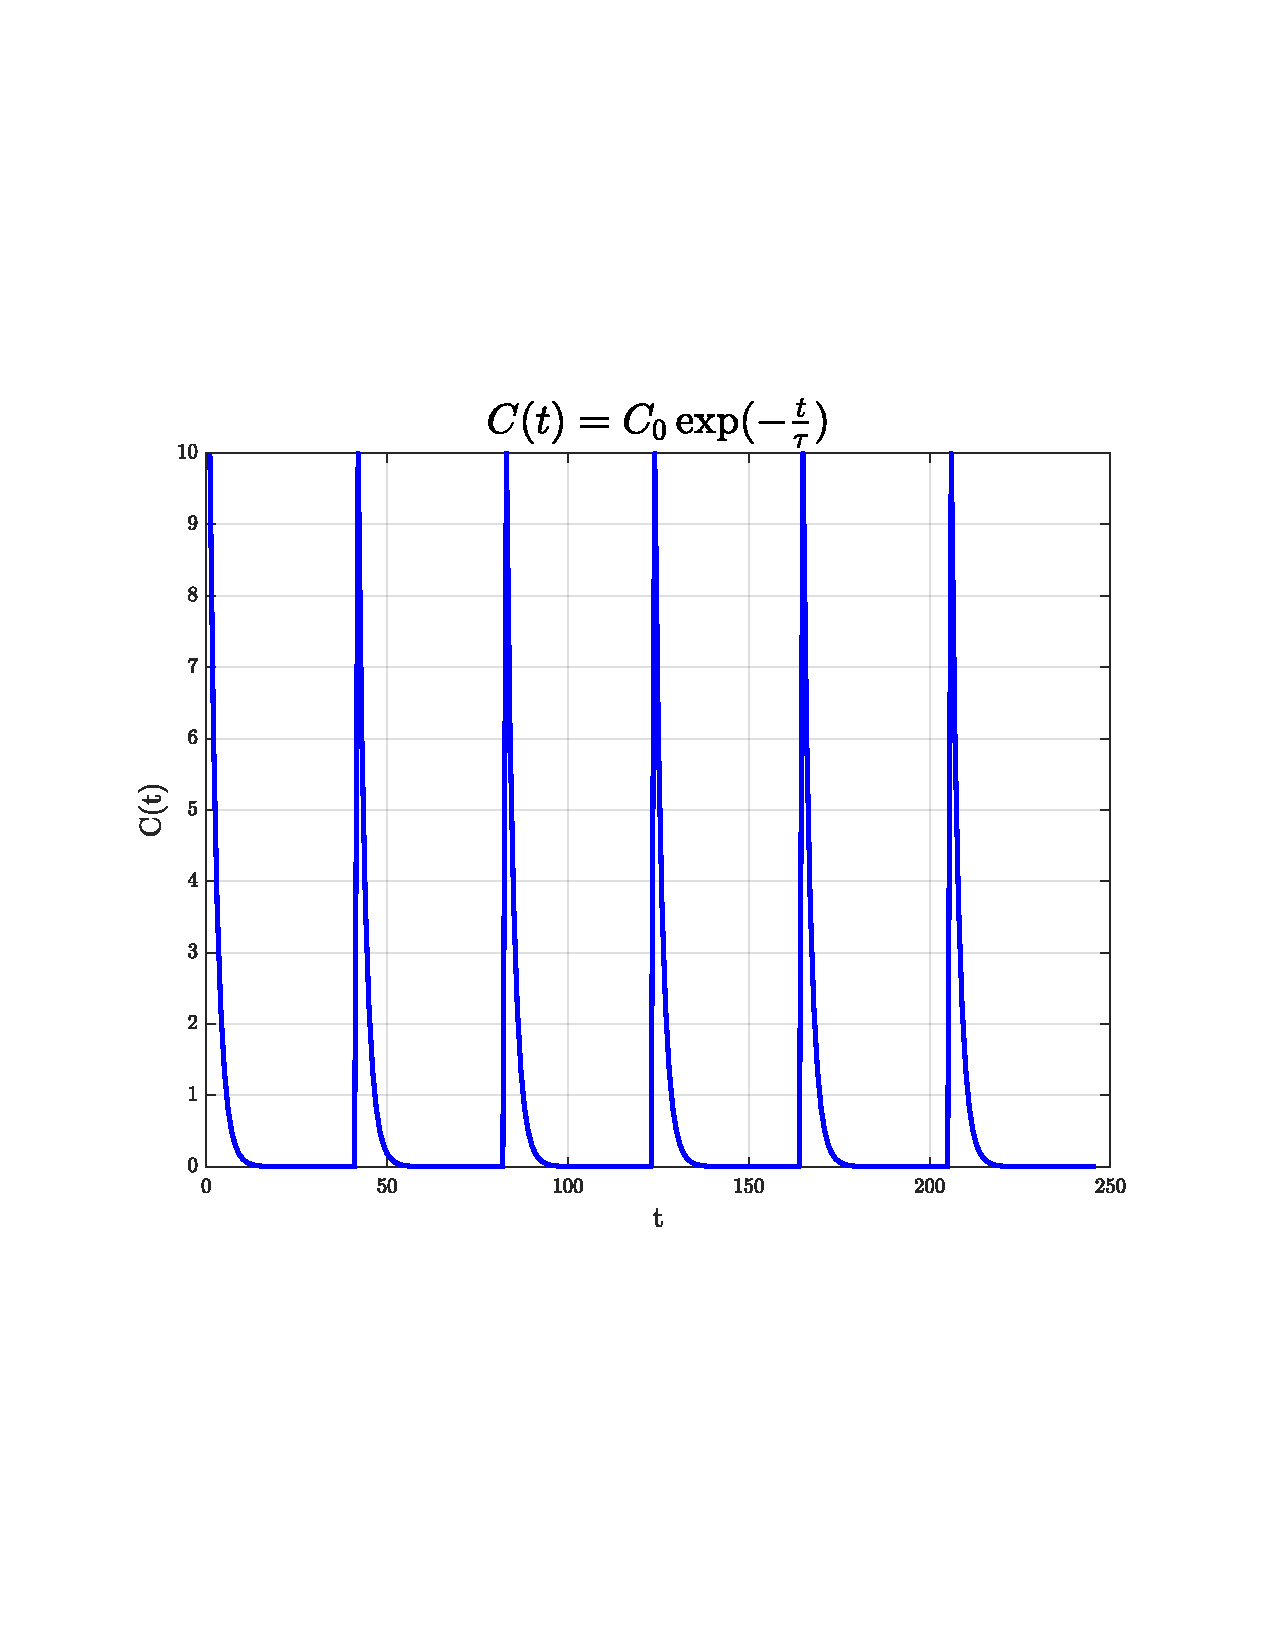
\includegraphics[scale=0.3]{exp_tau}
  \vspace{-5em}
 \caption{}
\end{figure}


\item [(b)]

$f(t) = C_0 e^{-\frac{t}{\tau}}$ with period $T$, so
\ba
	a_0	&= \frac{2}{T} \int_0^T C_0 e^{-\frac{t}{\tau}} dt \\
		&= \frac{2 C_0}{T} (-\tau) [e^{-\frac{t}{\tau}}]_0^T \\
		&= -2 C_0 \frac{\tau}{T} [ e^{-\frac{T}{\tau}} - 1] \\
		&= 2 C_0 \frac{\tau}{T} (1 - e^{-\frac{T}{\tau}}) \\
\ea
If $\tau \ll T$ then $e^{-\frac{T}{\tau}} \approx 0$ and $a_0 \approx 2 C_0 \frac{\tau}{T}$.
\ba
	a_k	&=  \frac{2}{T} \int_0^T C_0 e^{-\frac{t}{\tau}} \cos{\frac{2 k \pi t}{T}}dt \\
		&=   \frac{2 C_0}{T} \int_0^T e^{-\frac{t}{\tau}} \cos{\frac{2 k \pi t}{T}}dt \\
\ea
Using integration by parts with $u= \cos{\frac{2 k \pi t}{T}}, du = - \frac{2 k \pi}{T} \sin{\frac{2 k \pi t}{T}}$ and $dv =  e^{-\frac{t}{\tau}}, v = (-\tau)  e^{-\frac{t}{\tau}}$:
\[
	\int_0^T e^{-\frac{t}{\tau}} \cos{\frac{2 k \pi t}{T}} dt	=   (-\tau)  [e^{-\frac{t}{\tau}} \cos{\frac{2 k \pi t}{T}}]_0^T - \frac{2 k \pi \tau}{T} \int_0^T e^{-\frac{t}{\tau}} \sin{\frac{2 k \pi t}{T}}  dt \\
\]
Using again integration by parts:
\[
 	\int_0^T e^{-\frac{t}{\tau}} \sin{\frac{2 k \pi t}{T}}  dt =  (-\tau)  [e^{-\frac{t}{\tau}} \sin{\frac{2 k \pi t}{T}}]_0^T + \frac{2 k \pi \tau}{T} \int_0^T e^{-\frac{t}{\tau}} \cos{\frac{2 k \pi t}{T}}  dt 
\]
So
\ba
	(1 + (\frac{2 k \pi \tau}{T}))^2 \int_0^T e^{-\frac{t}{\tau}} \cos{\frac{2 k \pi t}{T}} dt &= (-\tau)  [e^{-\frac{t}{\tau}} \cos{\frac{2 k \pi t}{T}}]_0^T  + \frac{2 k \pi \tau^2}{T}   [e^{-\frac{t}{\tau}} \sin{\frac{2 k \pi t}{T}}]_0^T  \\
																&= (-\tau)  [e^{-\frac{t}{\tau}} \cos{\frac{2 k \pi t}{T}}]_0^T  + 0 \\
																&= \tau (1 - e^{-\frac{T}{\tau}} ) \\
						 \int_0^T e^{-\frac{t}{\tau}} \cos{\frac{2 k \pi t}{T}} dt	&=  \frac{\tau} {1 + (\frac{2 k \pi \tau}{T})^2}  (1 - e^{-\frac{T}{\tau}} ) \\																
\ea
Substituting back into the expression found for $a_k$ yields
\ba
	a_k 	&= 2 C_0 \frac{\tau} {T} \frac{1} {1 + (\frac{2 k \pi \tau}{T})^2} (1 - e^{-\frac{T}{\tau}} ) \\
		&=  2 C_0 \frac{\tau T} {T^2 + (2 k \pi \tau)^2}  (1 - e^{-\frac{T}{\tau}} ) \\
\ea
With the same assumption $\tau \ll T$ then $e^{-\frac{T}{\tau}} \approx 0$ and $a_k \approx 2 C_0 \frac{\tau} {T} \frac{1} {1 + (\frac{2 k \pi \tau}{T})^2}$.
Similarly to compute $b_k$
\ba
	b_k	&=  \frac{2}{T} \int_0^T C_0 e^{-\frac{t}{\tau}} \sin{\frac{2 k \pi t}{T}}dt \\
		&=   \frac{2 C_0}{T} \int_0^T e^{-\frac{t}{\tau}} \sin{\frac{2 k \pi t}{T}}dt \\
		&=   \frac{2 C_0}{T} \frac{2 k \pi \tau}{T} \int_0^T e^{-\frac{t}{\tau}} \cos{\frac{2 k \pi t}{T}}  dt \\
		&=   \frac{2 C_0}{T} \frac{2 k \pi \tau}{T} \frac{\tau} {1 + (\frac{2 k \pi \tau}{T})^2}  (1 - e^{-\frac{T}{\tau}} ) \\
		&=	4 C_0 k \pi \frac{\tau^2} {T^2 + (2 k \pi \tau)^2}  (1 - e^{-\frac{T}{\tau}} ) \\
\ea
Once again, since $e^{-\frac{T}{\tau}} \approx 0$ then $b_k \approx  	4 C_0 (\frac{\tau} {T})^2  \frac{1} {1 + (\frac{2 k \pi \tau}{T})^2}  \pi k$

\item [(c)]

For $k \ge 1$

\ba
	p_k	&= \frac{1}{2} (a_k^2 + b_k^2) \\
		&= \frac{1}{2} \bigg [ 4 C_0^2 (\frac{\tau} {T})^2  \frac{1} {(1 + (\frac{2 k \pi \tau}{T})^2)^2} + 
				16 C_0^2 (\frac{\tau} {T})^4   \frac{1} {(1 + (\frac{2 k \pi \tau}{T})^2)^2}  \pi^2 k^2 \bigg ] \\
		&= \frac{1}{2} 4 C_0^2  (\frac{\tau} {T})^2  \frac{1} {(1 + (\frac{2 k \pi \tau}{T})^2)^2}   \bigg [ 1 + 4  (\frac{\tau} {T})^2  \pi^2 k^2 \bigg ] \\			
		&= 2 C_0^2  (\frac{\tau} {T})^2  \frac{1} {(1 + (\frac{2 k \pi \tau}{T})^2)^2}   \bigg [ 1 + 4  (\frac{\tau} {T})^2  \pi^2 k^2 \bigg ] \\			
\ea

\item [(d)]
We have 
\[
	\frac{p_k}{2 ~ C_0^2} =  (\frac{\tau} {T})^2  \frac{1} {(1 + (\frac{2 k \pi \tau}{T})^2)^2}   \bigg [ 1 + 4  (\frac{\tau} {T})^2  \pi^2 k^2 \bigg ] 
\]

\begin{figure}[!h]
 \centering
 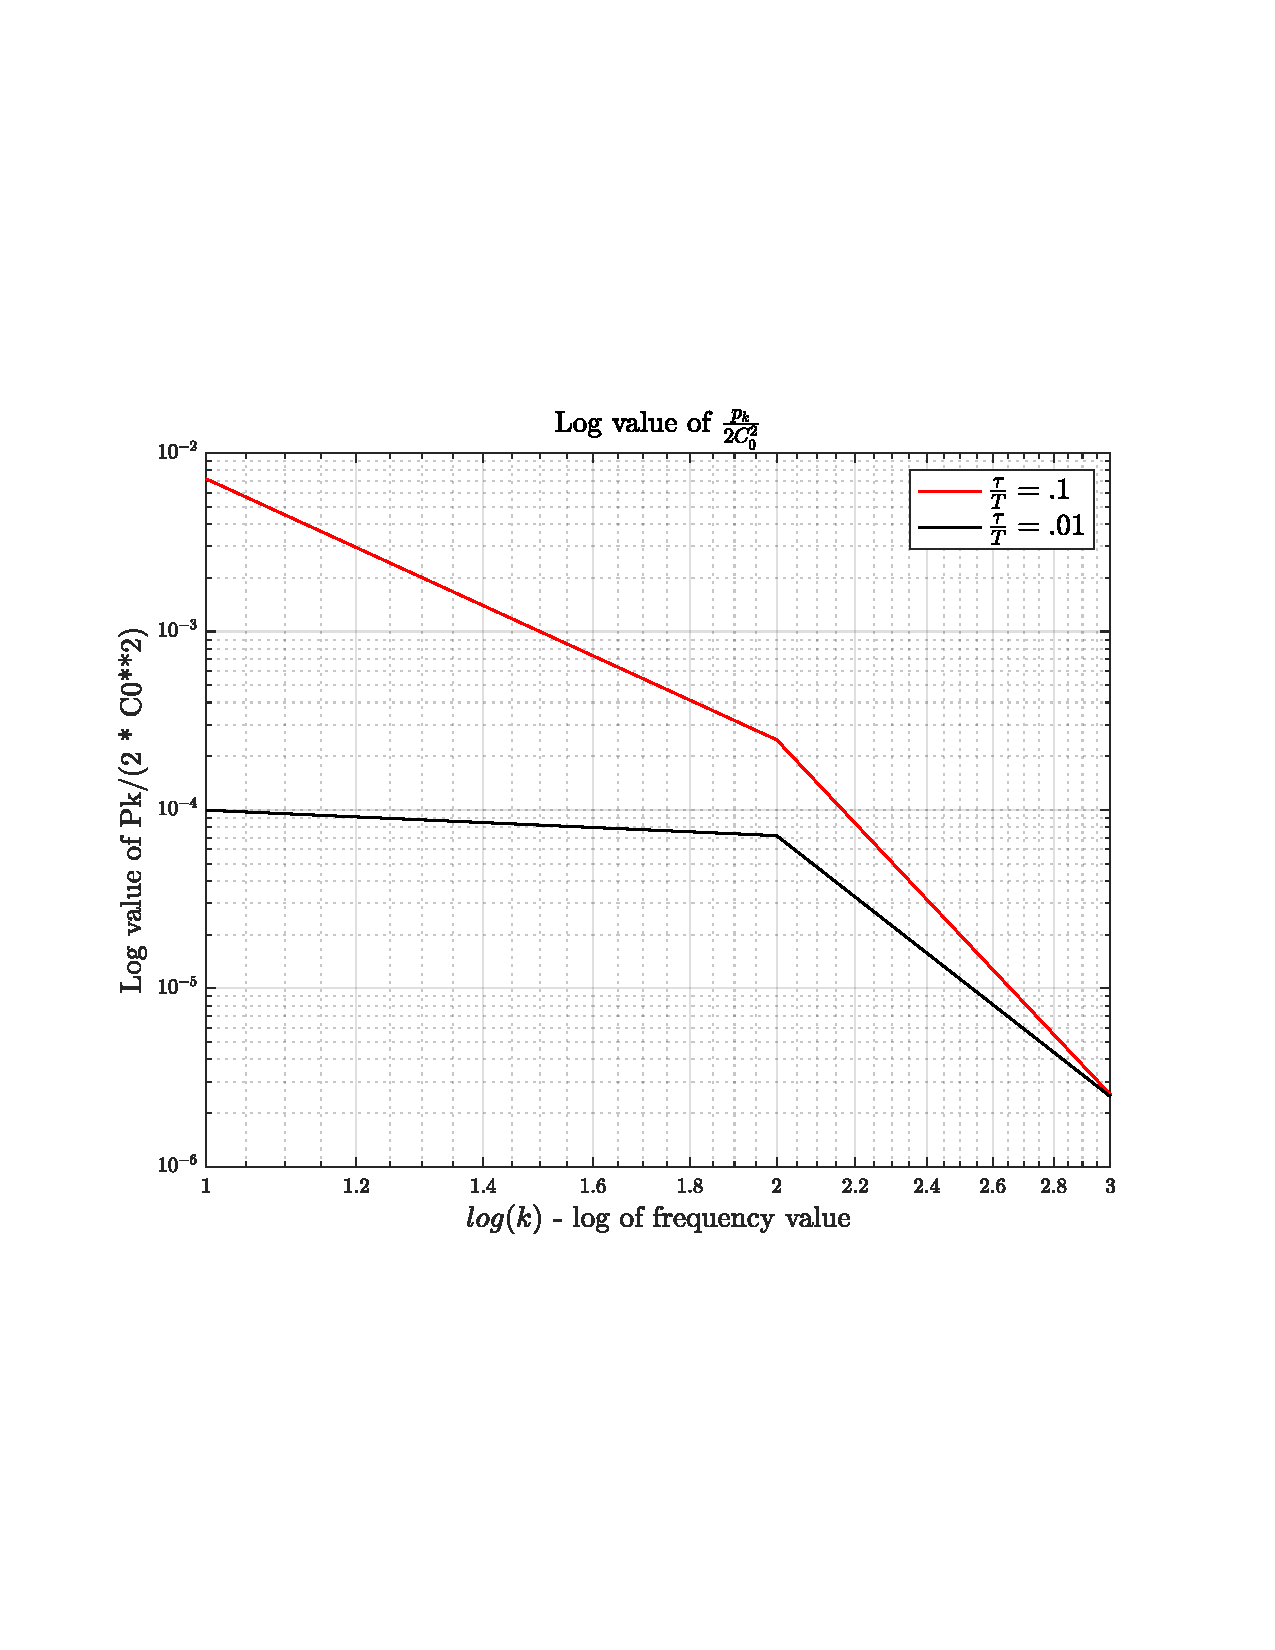
\includegraphics[scale=0.5]{power_vs_tau_T}
\end{figure}
From the plot we can see that the power $\frac{p_k}{2 ~ C_0^2}$ decreases as the frequency increases.
Power is close to $0$ starting with a frequency of $10$.

\item [(e)]
Looking at the plot in part (d), as the pulse $\tau$, becomes narrower, the power decreases linearly.
For a greater  $\frac{\tau}{T}$ , the power starts at a higher value  until an inflection point corresponding to frequency of $10$ ($1 = \log_{10}(10)$ on the graph).
Also for a higher $\frac{\tau}{T}$, the steepest the decrease in power. Eventually the two curves combine in one curve around
a frequency of ($2 = \log_{10}(100)$ on the graph).
The same observations are obtained with a loglog plot  of power  $\frac{p_k}{2 ~ C_0^2}$ vs.  $\frac{\tau}{T}$ for a frequency $k=10$. As the
pulses $\tau$ narrow or decrease the power decreases.

\begin{figure}[!h]
 \centering
 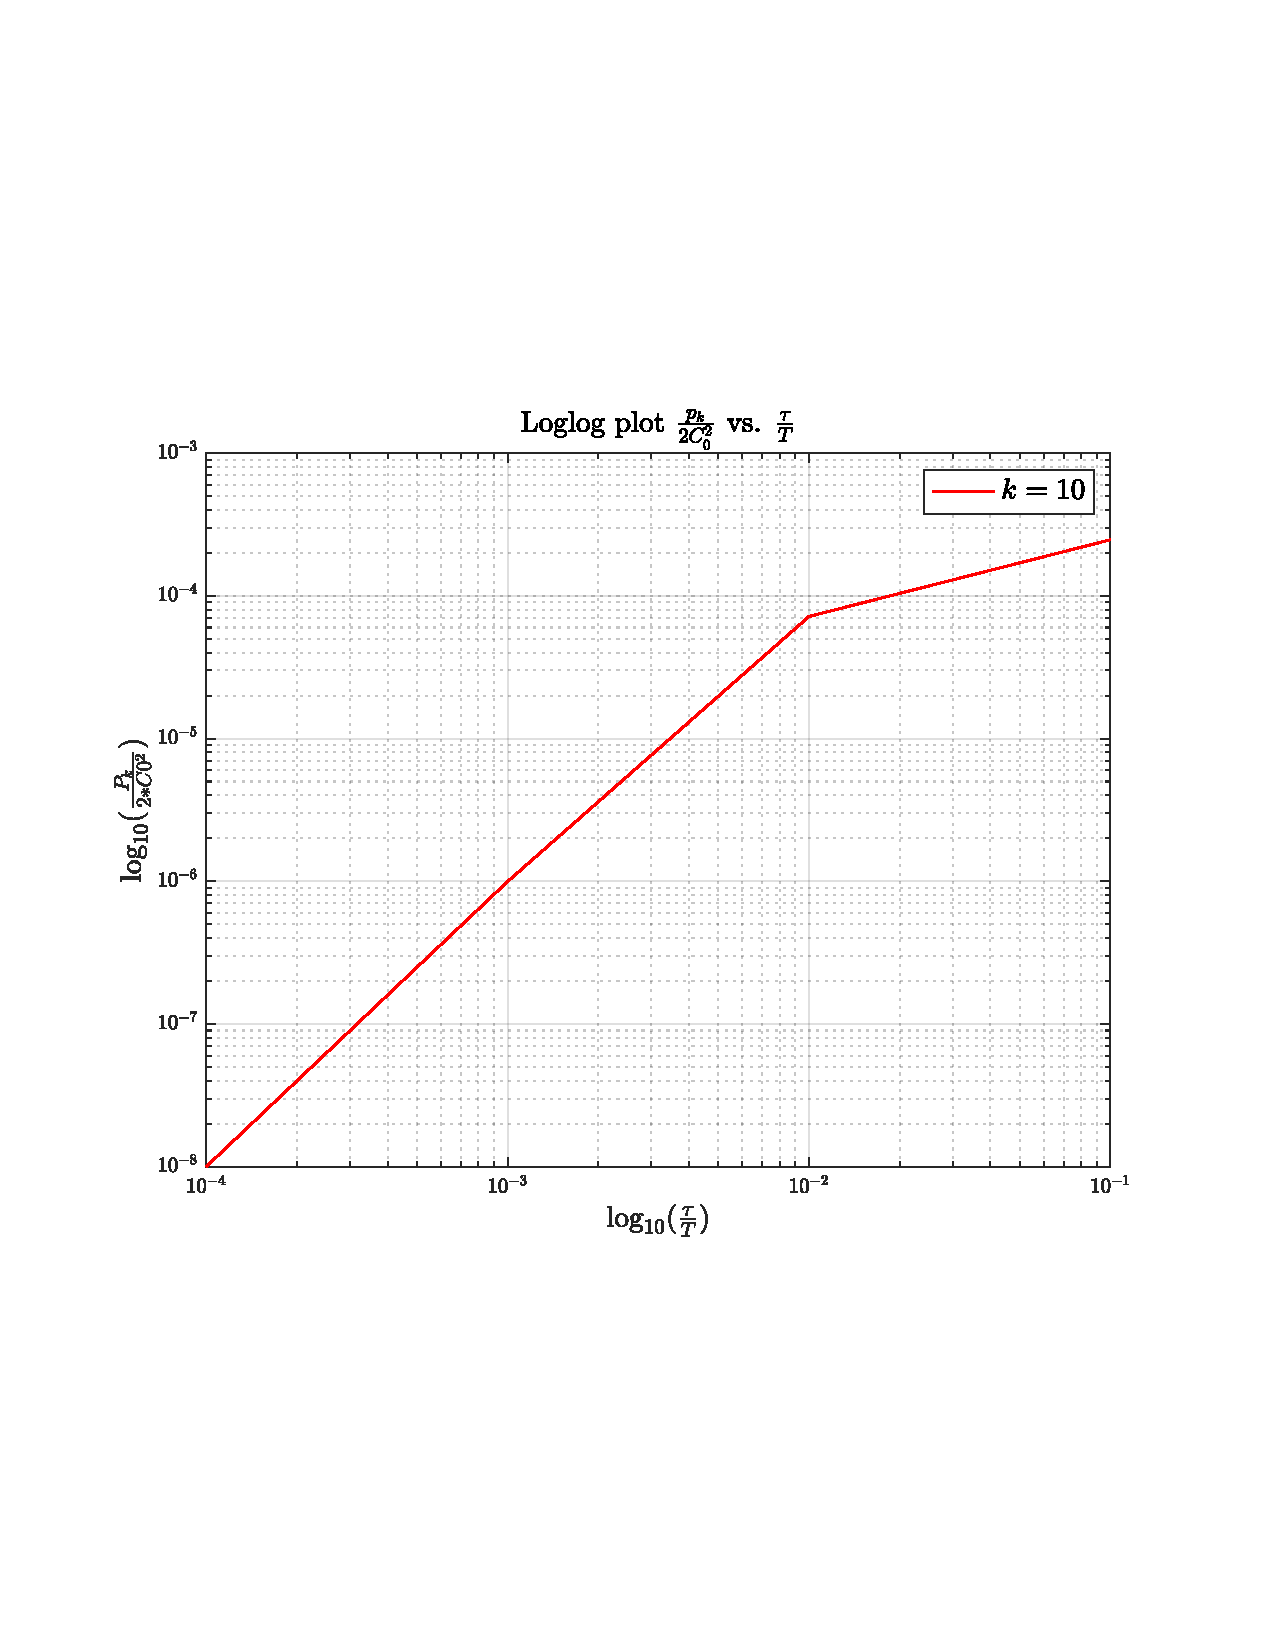
\includegraphics[scale=0.5]{power_vs_smaller_pulse}
\end{figure}


\item [(f)]
 We have
 \ba
 	a_k \cos(\frac{k 2 \pi t}{T}) + b_k \sin(\frac{k 2 \pi t}{T}) 	&= \cos(\phi_k) \cos(\frac{k 2 \pi t}{T}) + \sin(\phi_k) \sin(\frac{k 2 \pi t}{T}) \\
												&= \cos(\frac{k 2 \pi t}{T} - \phi_k) \\
 \ea
 where
 \ba
 	\tan(\phi_k) = \frac{\sin(\phi_k)} {\cos(\phi_k)} = \frac{b_k}{a_k}	&= 4 C_0 (\frac{\tau} {T})^2  \frac{1} {1 + (\frac{2 k \pi \tau}{T})^2}  \pi k  (2 C_0 \frac{\tau} {T} \frac{1} {1 + (\frac{2 k \pi \tau}{T})^2})^{-1} \\
													&= 2 \frac{\tau}{T} \pi k \\
											\phi_k	&= \arctan(2 \frac{\tau}{T} \pi k) \\
 \ea
 For $\frac{\tau}{T} = .1$, $\phi_1 \approx 32.14^{\circ}$  and $\phi_2 \approx 51.48^{\circ}$
 and for $\frac{\tau}{T} = .01$, $\phi_1 \approx 3.59^{\circ}$  and $\phi_2 \approx 7.16^{\circ}$

If we imagine a clock with a hand that turns at constant speed, making a full turn every $T$ seconds, and is pointing straight up at time $t=0$ when
the plasma rises to $C_0$. The phase $\phi_k$ is then the angle from the $12:00$ position to the current position and indicates how far is the next rise
in plasma concentration to $C_0$. For the same frequency (either $k=1$ or $k=2$), with a larger pulse we are closer to the next substance release.

\ee

\section*{Question 2}

\be
\item [(a)]
One simple way to describe $P(r)$ is to define it as $P(r) = A r + B$ with the conditions:
\ba
	A \cdot 0 + B &= Q \\
	A \cdot R + B &= 0 \\	
\ea
which gives $A=-\frac{Q}{R}$ and $B=Q$.
So
\ba
	P(r) =
	\begin{cases}
	Q (1 -\frac{r}{R}) ~ \text{ for } 0 \le r \le R\ \\
	0 ~ \text{ for }  r > R \\
	\end{cases} \\	
\ea


\begin{figure}[H]
 \centering
 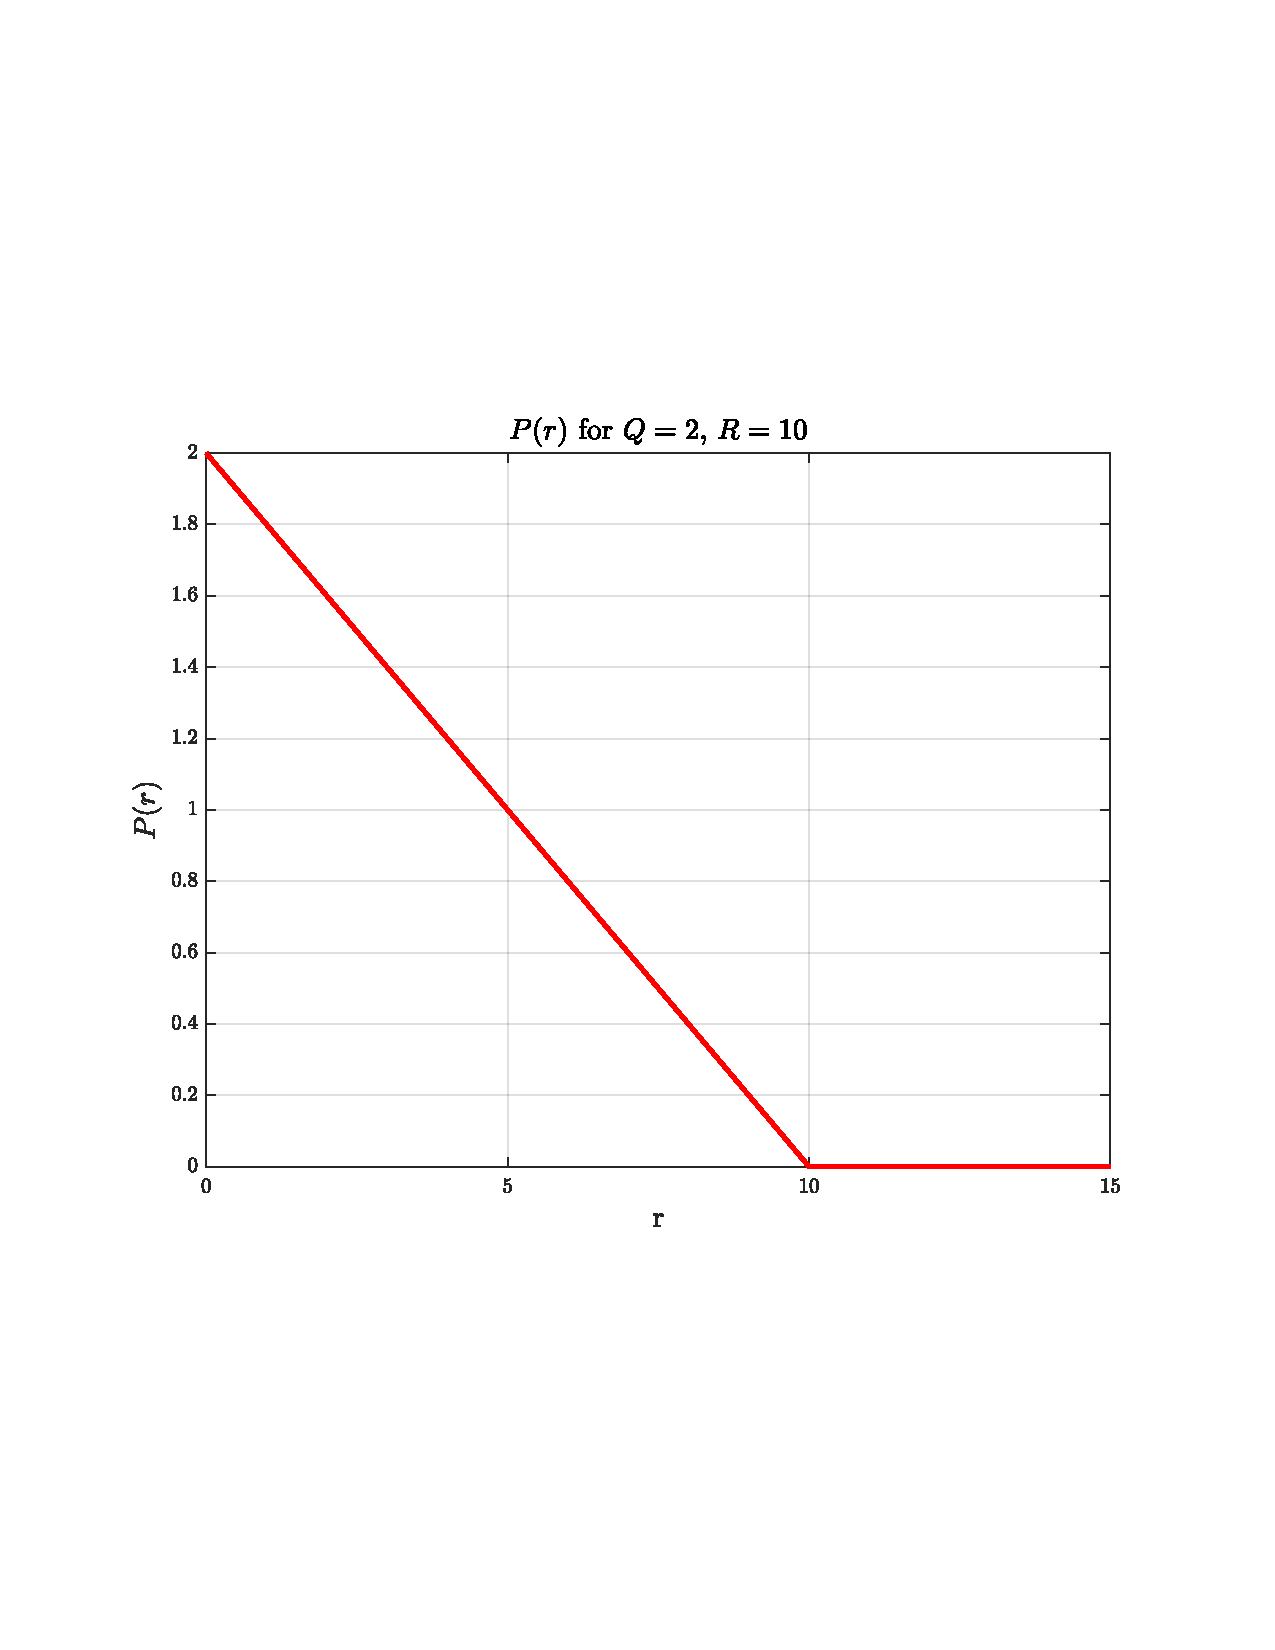
\includegraphics[scale=0.5]{pr}
\end{figure}
	

\item [(b)]

Since we assume no angular dependence: $\nabla^2 C = \frac {1}{r^2} \frac{d}{d r}(r^2 \frac{d C}{d r})$,  the differential equation is now:
\ba
	\frac{D}{r^2} \frac{d}{d r}(r^2 \frac{d C(r)}{d r}) +P(r)	&= 0 \\
	\frac{d}{d r}(r^2 \frac{d C(r)}{d r})				&= - \frac{r^2}{D} P(r) \\
\ea

\item [(c)]
Inside the cell $P(r) = Q (1 -\frac{r}{R})$, so we have to solve the differential equation
\ba
				\frac{d}{d r}(r^2 \frac{d C(r)}{d r})	&=  - \frac{r^2}{D} Q (1 -\frac{r}{R}) \\
											&=  \frac{Q}{D R } r^2 (r-R) \\
											&= \frac{Q}{D R } r^3 - \frac{Q}{D} r^2 \\
\ea
Integrating once
\ba
	r^2 \frac{d C(r)}{d r}	&=  \frac{Q}{4 D R } r^4 - \frac{Q}{3 D} r^3 + A  \\
	 \frac{d C(r)}{d r}	&=  \frac{Q}{4 D R } r^2 - \frac{Q}{3 D} r + \frac{A}{r^2} \\
\ea
Integrating again
\[
	 C_i(r)	=  \frac{Q}{12 D R } r^3 - \frac{Q}{6 D} r^2 - \frac{A}{r} + B ~ ~ A,B \text{:constants}, C_i \text{:inside cell concentration}
\]
Outside the cell $P(r)=0$ and we want to solve the differential equation
\[
				\frac{d}{d r}(r^2 \frac{d C(r)}{d r}) =  0
\]
Which by integration gives
\ba
	r^2 \frac{d C(r)}{d r} 		&= C_1 \\
	\frac{d C(r)}{d r}			&= \frac{C_1}{r^2} \\
	C_o(r)				&= -\frac{C_1}{r} + C_2 ~ ~ C_1,C_2 \text{:constants}, C_o \text{:outside cell concentration} \\
\ea

\item [(d)]

Applying the boundary conditions
\be
	\item [(i)]
	\[
		\lim_{r \rightarrow 0} C_i(r) = \lim_{r \rightarrow 0} \frac{Q}{12 D R } r^3 - \frac{Q}{6 D} r^2 - \frac{A}{r} + B
	\]
	since $\lim_{r \rightarrow 0} C_i(r) = \lim_{r \rightarrow 0} (- \frac{1}{r} + B) = \infty$ therefore to have finite concentration $C_i(r)$ at $r=0$ we need $A=0$
	
	\item [(ii)]
	\[
		\lim_{r \rightarrow \infty} C_o(r) = \lim_{r \rightarrow \infty} \bigg ( -\frac{C_1}{r} + C_2 \bigg ) = C_2
	\]
	The concentration goes to zero at infinity implies $C_2=0$
	
	\item [(iii)]
	We have now for $C_i(r)$ and $C_o(r)$:
	\ba
		C_i(r)	&=  \frac{Q}{12 D R } r^3 - \frac{Q}{6 D} r^2 + B \\
		C_o(r)	&= -\frac{C_1}{r}
	\ea
	$C_i(R) = C_o(R)$ and $\frac{d C_i(r)}{dr} = \frac{d C_o(r)}{dr} |_{r=R}$ yields
	\ba
		 \frac{Q}{12 D R } R^3 - \frac{Q}{6 D} R^2 + B 	&= -\frac{C_1}{R}\\
		 \frac{Q}{4 D} R - \frac{Q}{3 D} R 		&= \frac{C_1}{R^2}\\
	\ea
	Rearranging
	\ba
		 -\frac{Q}{12 D} R^2 + B 	&= -\frac{C_1}{R}\\
		 - \frac{Q}{12 D} R 		&= \frac{C_1}{R^2}\\
	\ea
	which gives
	\ba
		B 	&= \frac{Q}{6 D} R^2 \\
		C_1  &= -\frac{Q}{12 D} R^3 \\
	\ea	
	
substituting back
\ba
	C_i(r)	&=  \frac{Q}{12 D R } r^3 - \frac{Q}{6 D} r^2 +  \frac{Q}{6 D} R^2 \\
			&=  \frac{Q}{6 D } \bigg [ \frac{r^3}{2 R} - r^2 + R^2 \bigg ] \\
	C_o(r)	&= \frac{Q}{12 D} R^3 \frac{1}{r} \\
\ea
	
\ee

\item [(e)]
Knowing that  within the cell since $P(r)$ has maximum value $Q$ at $r=0$ and then it is zero for $r>R$,
we are looking for the value of $r$ for which $\frac{d C_i(r)}{d r}=0$:
\[
	\frac{d C_i(r)}{d r} = \frac{Q}{4 D R} r^2 - \frac{Q}{3 D} r = \frac{Q}{D} r (\frac{r}{4 R} - \frac{1}{3} )
\]
By the nature of the problem, the maximum concentration is at $r=0$:
\[
	C_M = \frac{Q}{6 D} R^2
\]
Inside the cell
\ba
	C_i(r)			&=  \frac{Q}{6 D} (\frac{1}{2} \frac{r^3}{R} - r^2 + R^2) \\
	\frac{C_i(r)}{C_M}	&= \frac{6 D}{Q}  R^{-2} \frac{Q}{6 D} (\frac{1}{2} \frac{r^3}{R} - r^2 + R^2) \\
					&=  \frac{1}{2} (\frac{r}{R})^3 -  (\frac{r}{R})^2 + 1 \\
\ea
And outside the cell 
\ba
	C_o(r)			&=   \frac{Q}{12 D} R^3 \frac{1}{r} \\
	\frac{C_o(r)}{C_M}	&=  \frac{6 D}{Q}  R^{-2}   \frac{Q}{12 D} R^3 \frac{1}{r}  \\
					&=  \frac{R}{2 r} \\
\ea

When the diffusion constant is doubled, the curve $\frac{C_i(r)}{C_M}$ stays the same since $\frac{C_i(r)}{C_M}$   does not depend on the diffusion constant $D$.

\begin{figure}[H]
 \centering
 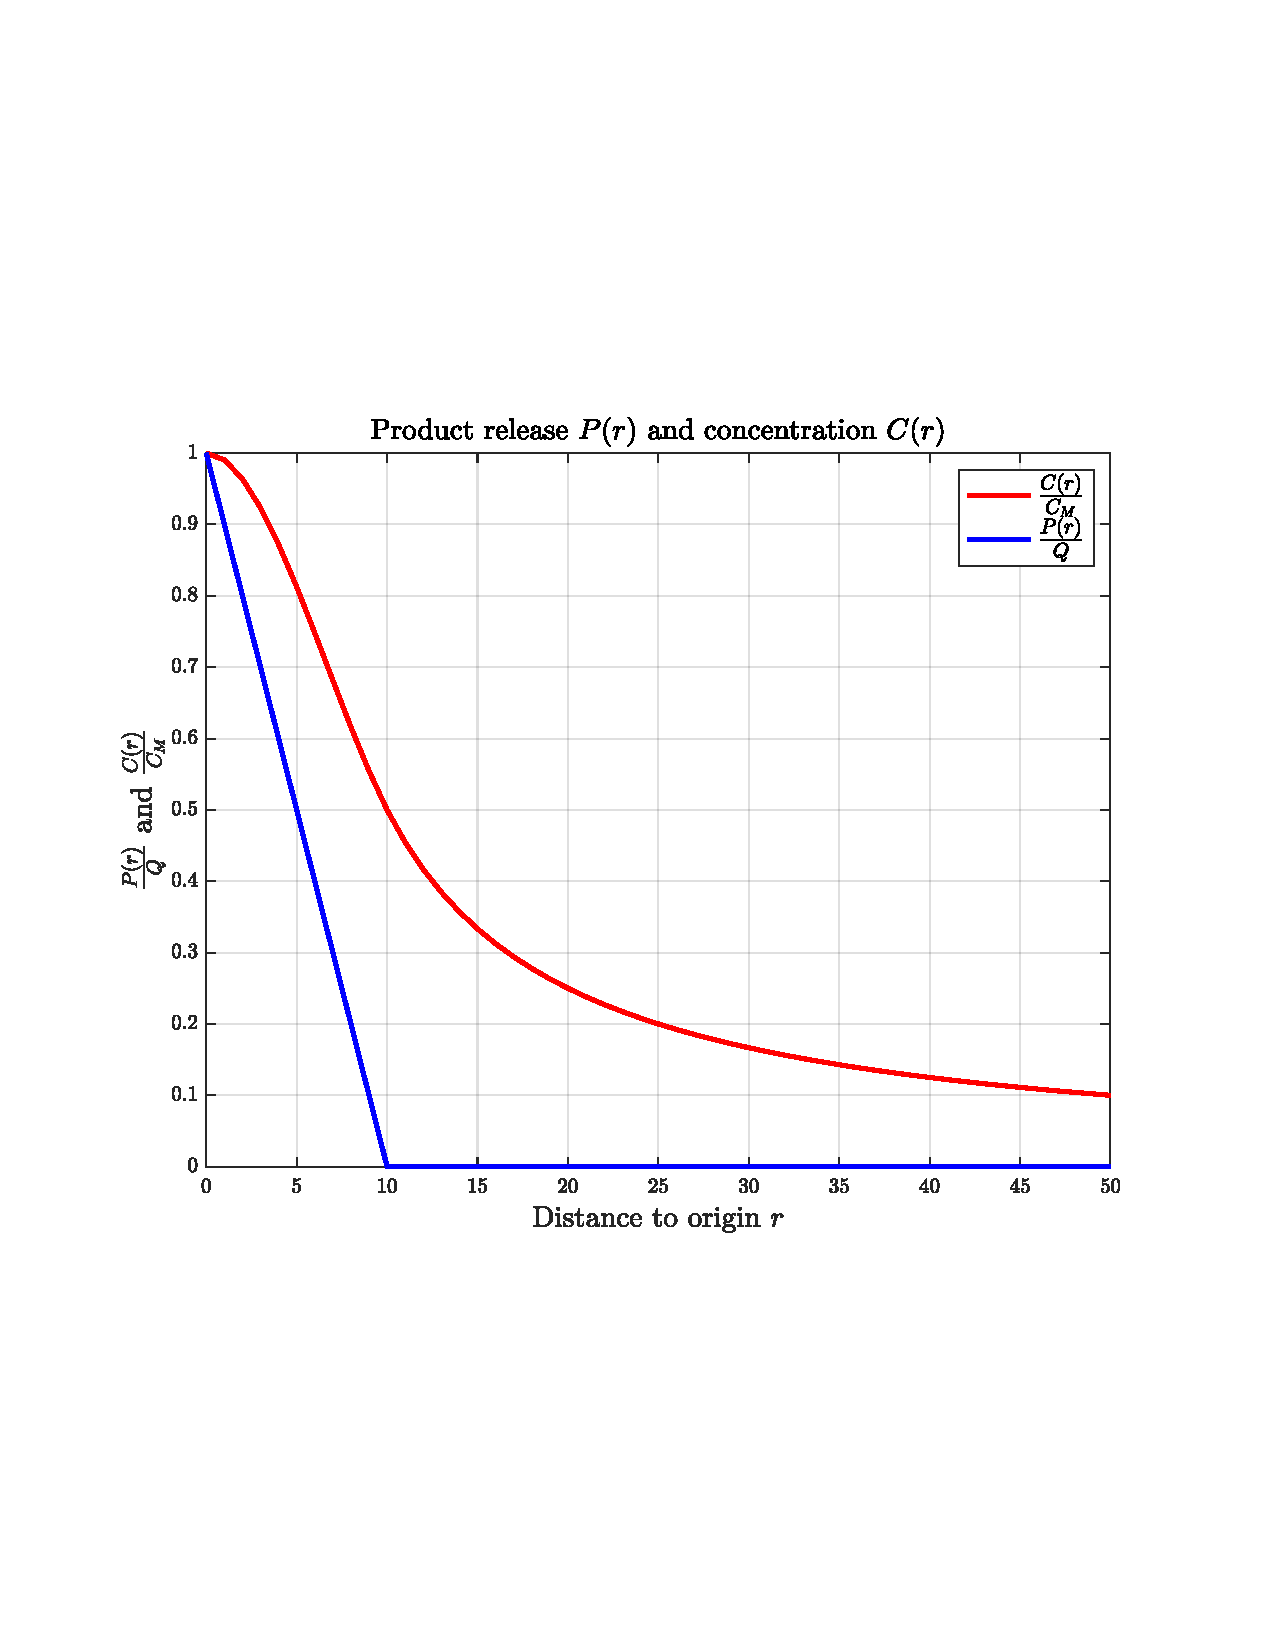
\includegraphics[scale=0.5]{concentration}
\end{figure}

However for arbitrary values of $Q$, $R$, and $D$ ($Q=1, R=10, D=1$), when the  diffusion constant $D$ is doubled,  the concentration curve is at a lower level
compared to the same concentration curve related to a diffusion constant $D$ as you can expect based on the expressions of $C_i(r)$ and $C_o(r)$ obtained above:

\begin{figure}[H]
 \centering
 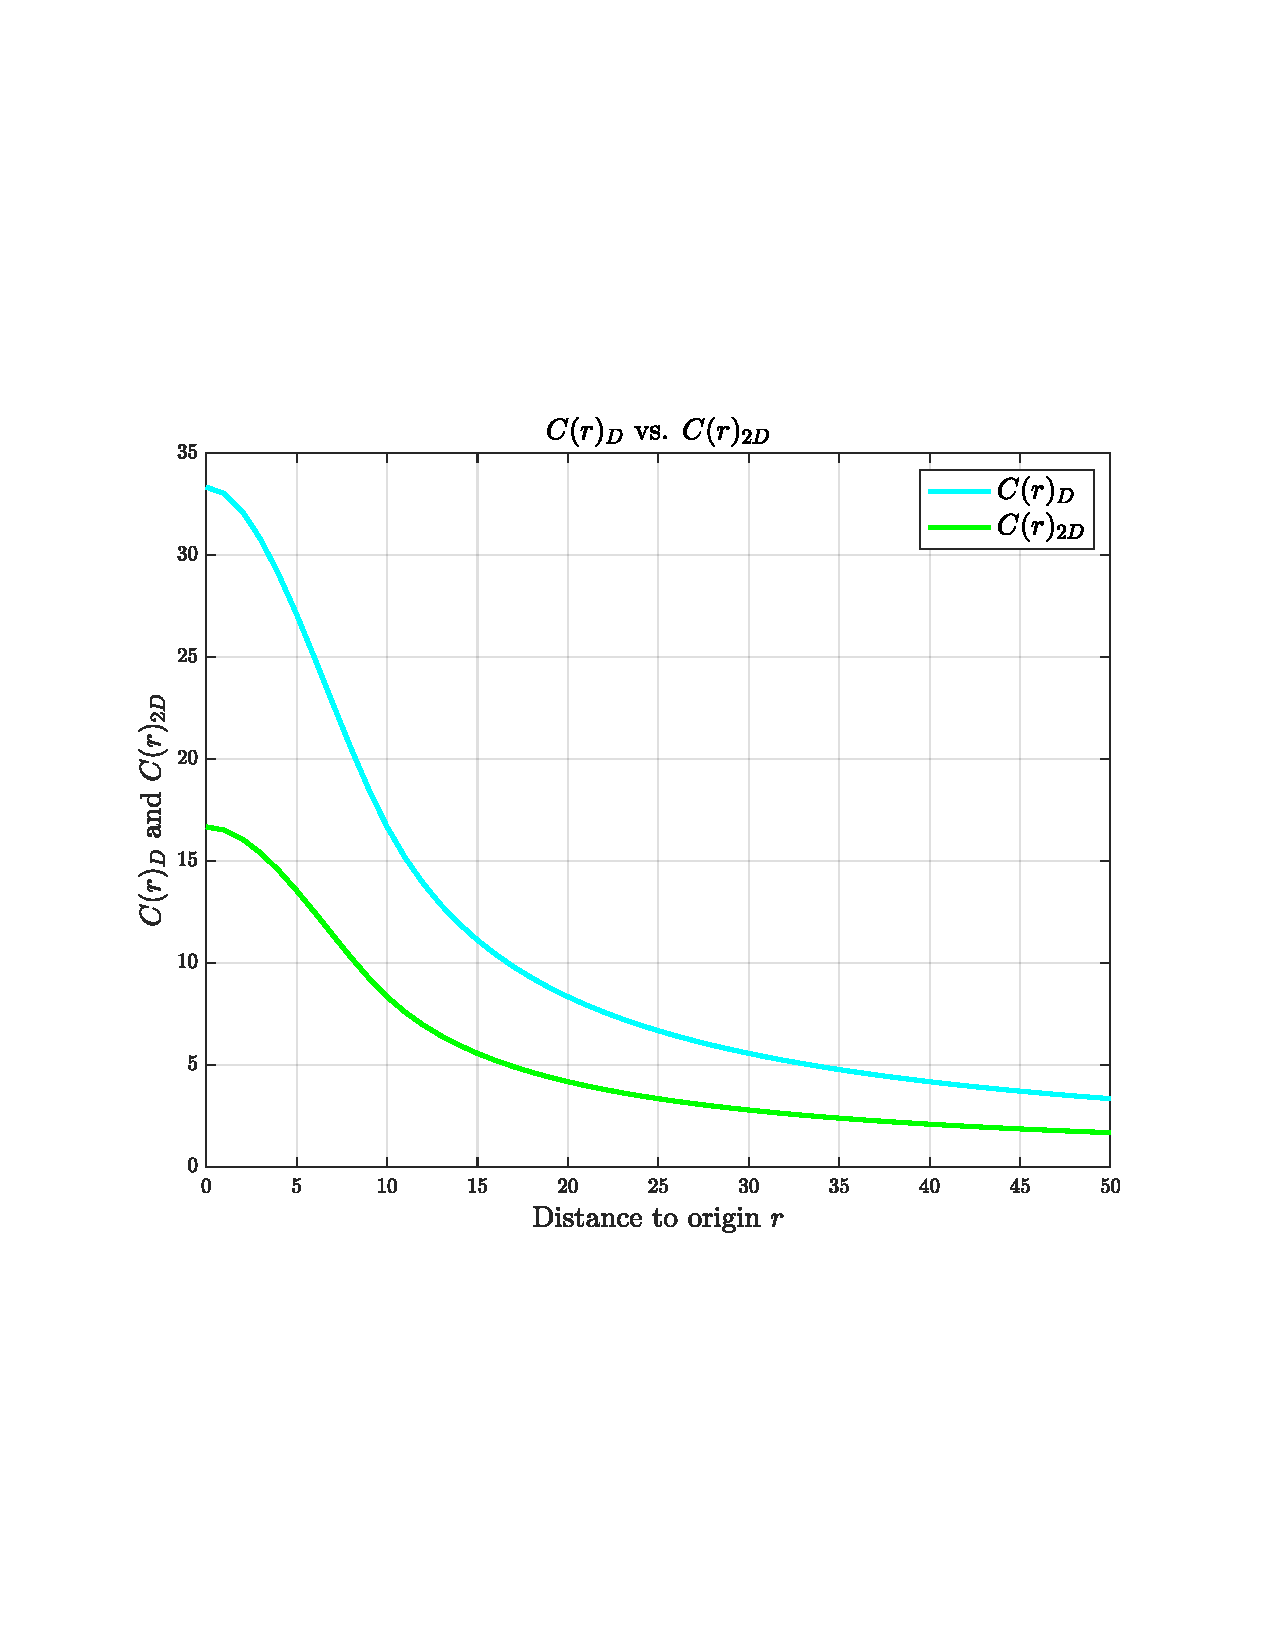
\includegraphics[scale=0.5]{concentration_d_2d}
\end{figure}

\ee

\end{document}
